\documentclass[11pt]{beamer}
\usetheme{Warsaw}
\usepackage[utf8]{inputenc}
%\usepackage[magyar]{babel}
\usepackage[T1]{fontenc}
\usepackage{amsmath}
\usepackage{amsfonts}
\usepackage{amssymb}
\usepackage{graphicx}
\usepackage{xurl}
\usepackage{multimedia}
\usepackage{xurl}
\author{Bendegúz Borkovits T7UR9P}
\title{Geant4 presentation 1}
%\setbeamercovered{transparent} 
%\setbeamertemplate{navigation symbols}{} 
%\logo{} 
\institute{Scientific Modeling Computer Laboratory} 
\date{February 2022} 
%\subject{} 
\begin{document}


\begin{frame}
\titlepage
\end{frame}

\begin{frame}{Tools and environment}
    \centering
    
\includegraphics[]{virtbox.png}
    
\includegraphics[scale = 0.1]{ubuntu-20-04-fossa.jpg} 
    \begin{itemize}
        \item Oracle VM VirtualBox (WSL + Xming was a failure)
        \item Ubuntu 20.04.3 LTS
        \item Geant4 building with cmake
    \end{itemize}
\end{frame}

\begin{frame}{Testing}
    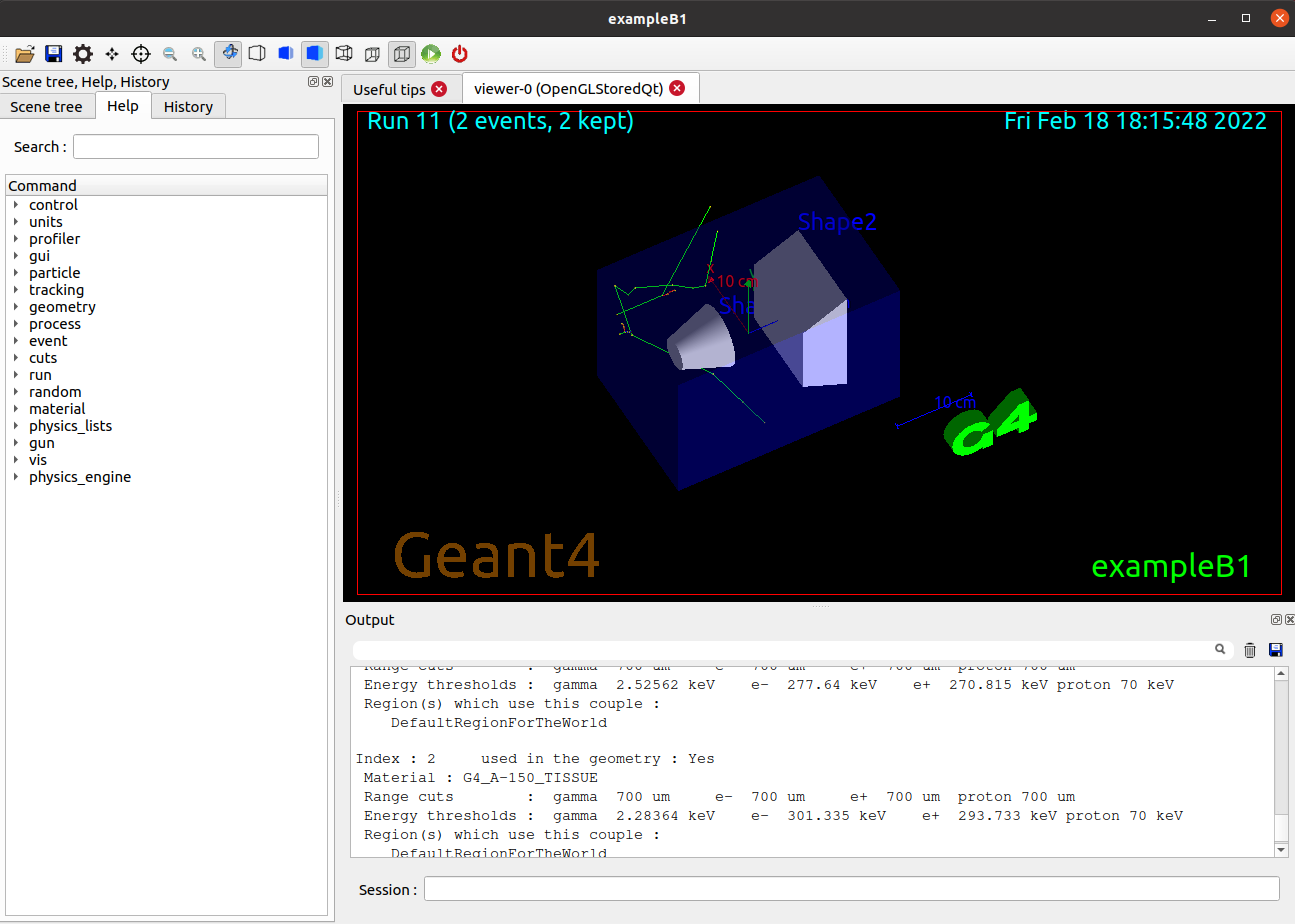
\includegraphics[scale=0.4]{geantkep.png}
\end{frame}

\begin{frame}{References}
    \begin{itemize}
    \item Oracle VM VirtualBox: \url{https://www.virtualbox.org/wiki/Downloads}
    \item Ubuntu 20.04: \url{https://ubuntu.com/download/desktop}
    \item Geant4: \url{https://geant4.web.cern.ch/support/download}
\end{itemize}
\end{frame}

\end{document}
